% no answer key
% \documentclass[letterpaper]{exam}

% answer key
\documentclass[letterpaper, landscape]{exam}
\usepackage{2in1, lscape} 
\printanswers

\usepackage{units} 
\usepackage{xfrac} 
\usepackage[fleqn]{amsmath}
\usepackage{cancel}
\usepackage{float}
\usepackage{mdwlist}
\usepackage{booktabs}
\usepackage{cancel}
\usepackage{polynom}
\usepackage{caption}
\usepackage{fullpage}
\usepackage{comment}
\usepackage{enumerate}
\usepackage{graphicx}
\usepackage{mathtools} 

\newcommand{\degree}{\ensuremath{^\circ}} 
\everymath{\displaystyle}

\title{Calculus I \\ Homework One \\ Section 1.1}
\author{}
\date{\today}

\begin{document}

  \maketitle

  \section{Homework}
    \begin{itemize*}
      \item read Section 1.1
      \item exercises: 1-2, 5-10, 12, 17-19, 21, 23, 26-31, 51-52, 57-58, 61-70
    \end{itemize*}

  \ifprintanswers
    \section{Solutions}
    \begin{description}

      \item[1]
        \begin{enumerate}[(a)]
          \item $f(-1) = \boxed{ -2 }$
          \item $f(2) \approx \boxed{ 2.8 }$
          \item $f(x) = 2$ when $\boxed{ x \approx \{-3, 1 \} }$
          \item $f(x) = 0$ when $\boxed{ x \approx \{ -2.5, 0.3 \} }$
          \item 
            \begin{itemize*}
              \item domain: $\boxed{ [-3, 3] }$
              \item range: $\boxed{ [-2, 3] }$
            \end{itemize*}

          \item $f$ is increasing on $\boxed{ (-1, 3) }$
        \end{enumerate}

      \item[2]
        \begin{enumerate}[(a)]
          \item $f(-4) = \boxed{ -2 }$; $g(3) = \boxed{ 4 }$

          \item $f(x) = g(x)$ when $\boxed{ x = \pm 2 }$

          \item $f(x) = -1$ when $\boxed{ x = \{ -3, 4 \} }$

          \item $f$ is decreasing on $\boxed{ (0, 4) }$

          \item 
            The domain and range of $f$ are:
            \begin{itemize*}
              \item domain: $\boxed{ [-4, 4] }$
              \item range: $\boxed{ [-2, 3] }$
            \end{itemize*}

          \item 
            The domain and range of $g$ are:
            \begin{itemize*}
              \item domain: $\boxed{ [-4, 3] }$
              \item range: $\boxed{ [0.5, 4] }$
            \end{itemize*}
        \end{enumerate}

      \item[5] not a function

      \item[6] 
        \begin{itemize*}
          \item domain: $\boxed{ [-2, 2] }$
          \item range: $\boxed{ [-1, 2] }$
        \end{itemize*}

      \item[7] 
        \begin{itemize*}
          \item domain: $\boxed{ [-3, 2] }$
          \item range: $\boxed{ [-3, 3] }$
        \end{itemize*}

      \item[8] not a function

      \item[9] This is probably the graph of Robinson Crusoe's weight over time.
        When he was 30 years old, he was stranded on a desert island for five
        years and had to subsist on a diet of coconuts which resulted in a
        dramatic weight loss. After he was rescued, he spent most of his time
        at Ben and Jerry's and rapidly gained back all the weight he'd lost
        while marooned.

      \item[10]
        He overslept and so he had to speed to his first appointment. He spent
        some time making a sale and then had a leisurely trip to his next
        appointment. After that he got lost and drove in circles for a little
        while before he found his next destination. He made another sale, and
        then took the freeway home.

      \item[12] The graph should look something like a sine wave, with a maximum at
        the summer solstice (July 21), a minimum at the winter solstice
        (December 21) and midway points at the two equinoxes (May 21 and
        September 21).

      \item[17] This should look like a sawtooth where the value climbs in a
        straight line to Wednesday and then drops back to close to zero every
        Wednesday.

      \item[18]
        \begin{enumerate}[(a)]
          \item $x(t)$ is a straight line with a slope of 400, aside from
            landing and takeoff, where the slope is a bit less.

          \item $y(t)$ is a straight line up to cruising altitude, then a
            horizontal line at cruising altitude, then a straight line back to
            ground level.

          \item The ground speed is a straight line at 400 for the flight, with
            some lower values for takeoff and landing.

          \item The vertical velocity is positive on takeoff, negative on
            landing, and 0 in between.
        \end{enumerate}

      \item[19] 
        \begin{figure}[H]
          \centering
          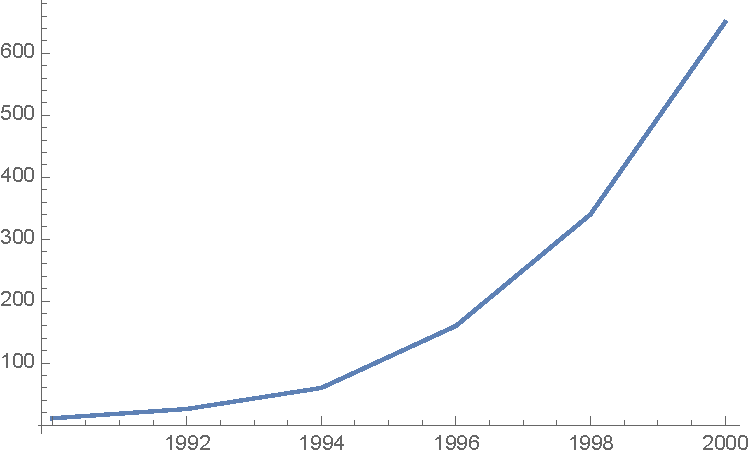
\includegraphics[scale = 0.6]{ex19.pdf}
          \caption{Exercise 19}
          \label{fig:ex19}
        \end{figure}

        \begin{enumerate}[(a)]
          \item see Figure \ref{fig:ex19}
          \item $f(1995) \approx 100$; $f(1999) \approx 500$
        \end{enumerate}

      \item[21]
        \begin{align*}
          f(2)          &= 12 \\
          f(-2)         &= 16 \\
          f(a)          &= 3a^2 - a + 2 \\
          f(-a)         &= 3a^2 + a + 2 \\
          f(a + 1)      &= 3a^2 + 5a + 4 \\
          f(2 f(a))     &= 6a^2 - 2a + 4 \\
          f(2a)      &= 12a^2 - 2a + 2 \\
          f(a^2)     &= 3a^4 - a^2 + 2 \\
          [ f(a) ]^2 &= 9a^4 - 6a^3 + 13a^2 - 4a +  4 \\
          f(a + h)   &= 3a^2 + 6ah + 3h^2 - a - h + 2 \\
        \end{align*}

      \item[23] $-h - 3$

      \item[26] $-\frac{1}{x+1}$

      \item[27]
        \begin{align*}
          3x - 1 & \neq 0 \\
          x      & \neq \frac{1}{3}
        \end{align*}

      \item[28]
        \begin{align*}
          x^2 + 3x + 2    & \neq 0 \\
          (x + 2) (x + 1) & \neq 0 \\
          x               & \neq \{-1, -2\} \\
        \end{align*}

      \item[29] $[0, \infty)$

      \item[30] $[0, 4]$

      \item[31] $(-\infty, 0) \cup (5, \infty)$

      \item[51]
        \begin{align*}
          2x + 2y & = 20 \\
          A       & = xy \\
          \\
          A(x)    & = 10x - x^2 \\
        \end{align*}

      \item[52]
        \begin{align*}
          xy & = 16 \\
          P  & = 2x + 2y \\
          \\
          P(x)    & = 2x + \frac{32}{x} \\
        \end{align*}

      % \item[56]
      %   \begin{itemize*}
      %     \item The perimeter of the semicircle at the top is: $P_c = \pi x$
      %     \item The perimeter of the rectangle part is: $P_r = x + 2h$
      %     \item The total perimeter is $P = x + 2h + \pi x$. This perimeter is 30:
      %   \end{itemize*}

      %   Since we know the perimeter is 20, we can find the height in terms of $x$: 
      %   \begin{align*}
      %     x + 2h + \pi x & = 20 \\
      %     h              & = 10-\frac{1 + \pi}{2} x \\
      %   \end{align*}

      %   \begin{itemize*}
      %     \item The area of the semicircle is: $A_c = \frac{\pi  x^2}{8}$
      %     \item The area of the rectangle is $A_r = xh$
      %     \item The total area is: $A = xh + \frac{\pi  x^2}{8}$
      %   \end{itemize*}

      %   Now we can use the expression for $h$ to get the area as a function of $x$:
      %   \begin{align*}
      %     A    & = xh + \frac{\pi  x^2}{8} \\
      %     A(x) & = x (10-\frac{1 + \pi}{2} x) + \frac{\pi  x^2}{8} \\
      %   \end{align*}

      \item[57]
        \begin{align*}
          V(x) & = x (12 - 2x) (20 - 2x) \\
               & = 4 x^3-64 x^2+240 x \end{align*}

      \item[58]
        If $d$ is in tenths of a mile, the cost in dollars is: 
        
        \[
          C(d) = 
            \begin{cases}
              2                & \text{if } d \leq 10 \\
              2 + 0.2 (d - 10) & \text{if } d > 10 \\
            \end{cases}
        \]

        \begin{figure}[H]
          \centering
          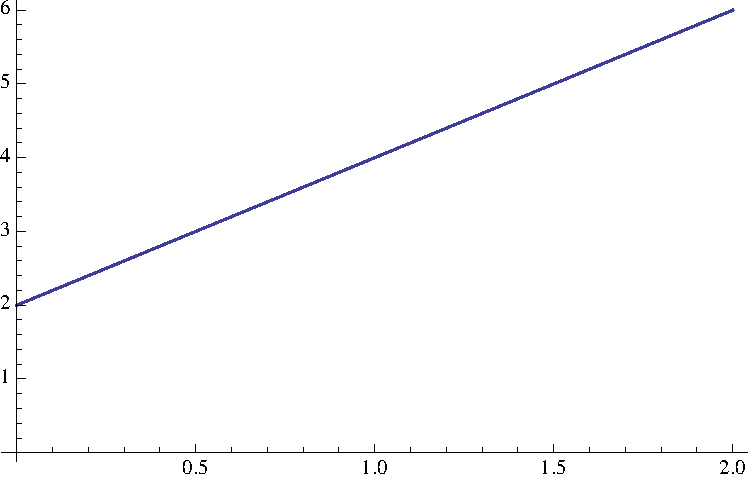
\includegraphics[scale = 0.8]{ex58.pdf}
          \caption{Exercise 58}
          \label{fig:ex58}
        \end{figure}

      \item[61] $f$ is odd and $g$ is even 

      \item[62] $f$ is neither and $g$ is even

      \item[63]
        \begin{enumerate}[(a)]
          \item $(-5, 3)$
          \item $(-5, -3)$
        \end{enumerate}

      \item[64]
        \begin{enumerate}[(a)]
          \item symmetric around the y-axis
          \item symmetric around the origin
        \end{enumerate}

      \item[65] odd
      \item[66] even
      \item[67] neither
      \item[68] odd
      \item[69] even
      \item[70] neither
        
    \end{description}

  \else
    \vspace{11 cm}
    \begin{quote}
      \begin{em}
         Do not worry about your difficulties in mathematics. I can assure you
         mine are still greater.
      \end{em}
    \end{quote}
    \hspace{1 cm} --Albert Einstein
  \fi

\end{document}

